%  LaTeX support: latex@mdpi.com
%  In case you need support, please attach all files that are necessary for compiling as well as the log file, and specify the details of your LaTeX setup (which operating system and LaTeX version / tools you are using).

% You need to save the "mdpi.cls" and "mdpi.bst" files into the same folder as this template file.

%=================================================================

\documentclass[computers,article,submit,moreauthors,pdftex,10pt,a4paper]{mdpi} 

%--------------------
% Class Options:
%--------------------
% journal
%----------
% Choose between the following MDPI journals:
% actuators, admsci, aerospace, agriculture, agronomy, algorithms, animals, antibiotics, antibodies, antioxidants, applsci, arts, atmosphere, atoms, axioms, batteries, behavsci, beverages, bioengineering, biology, biomedicines, biomimetics, biomolecules, biosensors, brainsci, buildings, c, cancers, catalysts, cells, challenges, chemosensors, children, chromatography, climate, coatings, computation, computers, condensedmatter, cosmetics, cryptography, crystals, data, dentistry, diagnostics, diseases, diversity, econometrics, economies, education, electronics, energies, entropy, environments, epigenomes, fermentation, fibers, fishes, fluids, foods, forests, futureinternet, galaxies, games, gels, genealogy, genes, geosciences, geriatrics, healthcare, horticulturae, humanities, hydrology, informatics, information, infrastructures, inorganics, insects, instruments, ijerph, ijfs, ijms, ijgi, inventions, jcdd, jcm, jdb, jfb, jfmk, jimaging, jof, jintelligence, jlpea, jmse, jpm, jrfm, jsan, land, languages, laws, life, literature, lubricants, machines, magnetochemistry, marinedrugs, materials, mathematics, medsci, medicines, membranes, metabolites, metals, microarrays, micromachines, microorganisms, minerals, molbank, molecules, mps, nanomaterials, ncrna, neonatalscreening, nutrients, particles, pathogens, pharmaceuticals, pharmaceutics, pharmacy, philosophies, photonics, plants, polymers, processes, proteomes, publications, recycling, religions, remotesensing, resources, risks, robotics, safety, sensors, sexes, sinusitis, socsci, societies, soils, sports, standards, sustainability, symmetry, systems, technologies, toxics, toxins, universe, vaccines, vetsci, viruses, water
%---------
% article
%---------
% The default type of manuscript is article, but can be replaced by: 
% addendum, article, bookreview, briefreport, casereport, changes, comment, commentary, communication, conceptpaper, correction, conferencereport, meetingreport, creative, datadescriptor, discussion, editorial, essay, erratum, hypothesis, interestingimage, letter, newbookreceived, opinion, obituary, projectreport, reply, retraction, review, shortnote, supfile, technicalnote
% supfile = supplementary materials
%----------
% submit
%----------
% The class option "submit" will be changed to "accept" by the Editorial Office when the paper is accepted. This will only make changes to the frontpage (e.g. the logo of the journal will get visible), the headings, and the copyright information. Journal info and pagination for accepted papers will also be assigned by the Editorial Office.
%------------------
% moreauthors
%------------------
% If there is only one author the class option oneauthor should be used. Otherwise use the class option moreauthors.
%---------
% pdftex
%---------
% The option "pdftex" is for use with pdfLaTeX. If eps figure are used, use the option "dvipdfmx", with LaTeX and dvi2pdf.

%=================================================================
\firstpage{1} %%MDPI internal note: new layout%%
\makeatletter %%MDPI internal note: new layout%%
\setcounter{page}{\@firstpage} %%MDPI internal note: new layout%%
\makeatother %%MDPI internal note: new layout%%
\articlenumber{x}
\doinum{10.3390/------}
\pubvolume{xx}
\pubyear{2016}
\copyrightyear{2016}
\externaleditor{Academic Editor: name}
\history{Received: date; Accepted: date; Published: date}
%------------------------------------------------------------------
% The following line should be uncommented if the LaTeX file is uploaded to arXiv.org
%\pdfoutput=1

%=================================================================

\usepackage{comment}
\usepackage{url}

\usepackage{amsmath}
\usepackage{graphicx}
\usepackage{subcaption}
\usepackage{multirow}
\usepackage{caption}

\usepackage{listings}

\usepackage{algorithm}% http://ctan.org/pkg/algorithms
\usepackage{algpseudocode}% http://ctan.org/pkg/algorithmicx


\lstset{
	aboveskip=0.5\baselineskip,
	belowskip=0.5\baselineskip,
	tabsize=2,
	upquote=true,
	basicstyle=\small,
	columns=fixed,
	showstringspaces=false,
	mathescape,
	breaklines=true,
	frame=single,
	showtabs=false,
	showspaces=false,
	showstringspaces=false,
	identifierstyle=\ttfamily,
	keywordstyle=\ttfamily
}


% Add packages and commands here. The following packages are loaded in our class file: fontenc, calc, indentfirst, fancyhdr, graphicx, lastpage, ifthen, lineno, float, amsmath, setspace, enumitem, mathpazo, eulervm, booktabs, titlesec, amsthm, hyphenat, natbib, hyperref, footmisc, geometry, caption, url,

%=================================================================
%% Please use the following mathematics environments:
 \theoremstyle{mdpi}
 \newcounter{thm}
 \setcounter{thm}{0}
 \newcounter{ex}
 \setcounter{ex}{0}
 \newcounter{re}
 \setcounter{re}{0}

 \newtheorem{Theorem}[thm]{Theorem}
 \newtheorem{Lemma}[thm]{Lemma}
 \newtheorem{Corollary}[thm]{Corollary}
 \newtheorem{Proposition}[thm]{Proposition}

 \theoremstyle{mdpidefinition}
 \newtheorem{Characterization}[thm]{Characterization}
 \newtheorem{Property}[thm]{Property}
 \newtheorem{Problem}[thm]{Problem}
 \newtheorem{Example}[ex]{Example}
 \newtheorem{ExamplesandDefinitions}[ex]{Examples and Definitions}
 \newtheorem{Remark}[re]{Remark}
 \newtheorem{Definition}[thm]{Definition}
%% For proofs, please use the proof environment (the amsthm package is loaded by the MDPI class).

%=================================================================
% Full title of the paper (Capitalized)
\Title{High performance encapsulation and networking in Casanova 2}

% Authors (Add full first names)
\Author{Francesco Di Giacomo $^{1}$, Mohamed Abbadi $^{1}$* , Agostino Cortesi $^{1}$, Pieter Spronck $^{2}$, Giulia Costantini $^{3}$ and Giuseppe Maggiore $^{3}$}
%\AuthorNames{} %%MDPI internal note: new layout%%

% Affiliations / Addresses (Add [1] after \address if there is only one affiliation.)
\address{%
$^{1}$ \quad Ca'Foscari University, Venice (Italy); \{francesco.digiacomo,mohamed.abbadi,cortesi\}@unive.it\\
$^{2}$ \quad Tilburg University, Tilburg (The Netherlands); p.spronck@uvt.nl\\
$^{3}$ \quad Hogeschool Rotterdam, Rotterdam (The Netherlands); \{costg,maggg\}@hr.nl}

% Contact information of the corresponding author
\corres{Correspondence: mohamed.abbadi@unive.it}


% Simple summary
%\simplesumm{} %%MDPI internal note: new layout%%

% Abstract (Do not use inserted blank lines, i.e. \\) 
\abstract{\textit{Encapsulation} is a programming technique that helps developers keeping code readable and maintainable. However, encapsulation in modern object oriented languages often causes significant runtime overhead. Developers must choose between clean encapsulated code or fast code. In the application domain of computer games, speed of execution is of utmost importance, which means that the choice between clean and fast usually is decided in favor of the latter. In this paper we discuss how encapsulation is embedded in the Casanova 2 game development language, and show how Casanova 2 allows developers to write encapsulated game code, which thanks to extensive optimization achieves at the same time high levels of performance. Furthermore, we show that the abstractions provided by Casanova so far cover no more than the tip of the iceberg: we document a further extension in the traditionally challenging domain of networking and show how the language can provide significant improvement in productivity.}

% Keywords
\keyword{Domain Specific Language; Encapsulation; Networking; Games}

% The fields PACS, MSC, and JEL may be left empty or commented out if not applicable
%\PACS{J0101}
%\MSC{}
%\JEL{}

% If this is an expanded version of a conference paper, please cite it here: enter the full citation of your conference paper, and add $^\S$ in the end of the title of this article.
%\conference{}

%%%%%%%%%%%%%%%%%%%%%%%%%%%%%%%%%%%%%%%%%%
% Only for the journal Data:

%\dataset{DOI number or link to the deposited data set in cases where the data set is published or set to be published separately. If the data set is submitted and will be published as a supplement to this paper in the journal Data, this field will be filled by the editors of the journal. In this case, please make sure to submit the data set as a supplement when entering your manuscript into our manuscript editorial system.}

%\datasetlicense{license under which the data set is made available (CC0, CC-BY, CC-BY-SA, CC-BY-NC, etc.)}

%%%%%%%%%%%%%%%%%%%%%%%%%%%%%%%%%%%%%%%%%%

\begin{document}

%%%%%%%%%%%%%%%%%%%%%%%%%%%%%%%%%%%%%%%%%%
%% Sections that are not mandatory are listed as such. The section titles given are for Articles. Review papers and other article types have a more flexible structure. 

%% Only for the journal Gels: Please place the Experimental Section after the Conclusions

%%%%%%%%%%%%%%%%%%%%%%%%%%%%%%%%%%%%%%%%%%
%\setcounter{section}{-1} %% Remove this when starting to work on the template.

\section{Introduction}
\label{sec:introduction}
The video games industry is an ever growing sector with sales surpassing 20 billion dollars in 2014 \cite{game_sales_esa}. Video games are not only built for entertainment purposes, but they are also used for Edutainment, Higher Education, Health Care, Corporate, Military, Research, and others \cite{CMP_Media_2004,serious_games}. These so-called \textit{serious games} usually do not enjoy the budgets available in the entertainment industry \cite{stapleton2004serious}. Therefore, developers of serious games are interested in tools capable of overcoming the coding difficulties associated with the complexity of games, and reducing the long development times.

Video games are composed of several inter-operating components, which accomplish different and coordinated tasks, such as drawing game objects, running the physics simulation of bodies, and moving non-playable characters using artificial intelligence. These components are periodically activated in turn to update the game state and draw the scene. When game complexity increases, this leads to an increase in size and complexity of components, which, in turn, leads to an increase in the complexity of developing and maintaining them, and thus an increase of development costs.

%As the components increases their complexity and size the difficulty to develop and maintain them increases as well\footnote{Because of the nature of games O-O languages lend themselves to easily define games\cite{neubauer2002object}}. This leads to higher complexity, thus to higher amount of costs.

A possible approach to reduce development costs is to use game development tools (e.g., GameMaker, Unity3D, or UnrealEngine \cite{petridis2010engine}), which tend to produce simple games that are hard to customize and bound to a specific genre. To provide some level of customization, game developers rely on general-purpose languages (GPLs) \cite{lewis2002game}. GPLs are typically unable to provide domain-specific abstractions and constructs. This means that when developing games by means of a GPL the resulting code will be complex and expensive to maintain \cite{Rocki:2014:FAP:2554850.2555029,sujeeth2014delite}. According to \cite{beck2000extreme}, the typical life cycle of software implemented by means of a GPL is: (\textit{\textbf{i}}) \underline{building a prototype}; (\textit{\textbf{ii}}) \underline{designing} a version in which the code is readable and maintainable; and eventually (\textit{\textbf{iii}}) \underline{refactoring}, after obtaining confidence with the context and the problem, the code from the previous point, so as to realize the last (often non-functional) requirements. 

We can see that the just introduced cycle is applicable to game development as well: (\textit{\textbf{i}}) building a \underline{game prototype} is always necessary to take confidence with the context of the problem and the chosen tool; (\textit{\textbf{ii}}) \underline{designing game code} that is maintainable and readable requires developers to abstract the problem and to focus more on the high-level interactions of the game and its data structures. Software development techniques have been studied to improve software maintainability and tackle complexity \cite{collar2006role}. Encapsulation, which consists of isolating a set of data and operations on those data within a module and providing precise specifications for the module \cite{citeulike:10949855}, is an example of a technique aimed at increasing code maintainability and readability; and (\textit{\textbf{iii}}) \underline{refactoring} is a common process in game development, see for example the case of performance optimization, which is of high importance for games, since it is strictly connected to game smoothness, i.e., to the game's frame rate, and smoothness strongly influences the perceived quality of a game \cite{claypool2009perspectives}. Indeed developing a game is a highly dynamic process \cite{takeuchi1986new} involving a wide variety of team members with different roles, such as designers, programmers, etc. Design very often changes during the development stage, as proven in several examples from the industry, such as Starcraft, Duke Nuke'em Forever, and Final Fantasy XV \cite{variety_article}. Small changes at the abstract design level translates into considerable amount of code, which might affect the overall architecture; thus every stage of the above life cycle requires effort and is time consuming. An example of this is when using encapsulation \cite{zhou2008partial} in the code. Since a game may feature many small entities, encapsulation forces those entities to interact through specific interfaces. When calling methods of the interfaces, overhead is added due to dynamic dispatching \cite{zhou2008partial}. Such overhead ultimately affects the performance of games at runtime negatively, so a complete refactoring that accommodates performance becomes necessary. Similar negative effects come from various design patterns, which all add layers of indirection. These effects impact negatively cache coherency and force CPU prediction failures. Traditional networking in games is another example that typically breaks encapsulation as the what to send over the network is dependent on the game logic; thus small changes in the game structure could affect heavily the networking layer.


What seems ideal is to have the advantages coming from both stages (\textit{ii}) and (\textit{iii}): game code that is well maintainable and readable, and at the same time with a fast run time. For this purpose, we investigated this problem and developed a solution that allows developers to write encapsulated code. Encapsulation is ``a language mechanism for restricting direct access to some of the object components.''. According to the definition of encapsulation, data and operations on them must be isolated within a module and a precise interface must be provided. Our solution turns, through extensive automated optimization, encapsulated code into an equivalent high-performance executable, therefore relieving developers from refactoring important design structures by hand, thus reducing the chances to make mistakes. As a further note, we want to underline that this optimization could be performed at source code level; however the logic of the program would be irremediably lost in the complex details of the architecture needed for the optimization, and thus debugging the code would be impractical. This is why we decided to look for a solution at a lower level of abstraction.


%\noindent
To sum up, in this paper we present a solution, which makes use of optimization transformations, that addresses the problem of the loss of performance in encapsulated games and of abstracting networking primitives. We present our solution as an extension for a domain specific language for games, called ``Casanova 2'', which allows developers to write high quality games at reduced development costs. 

%\subsection{Structure of the paper}
We start with a discussion about the focus of this paper\footnote{This paper is an extended version of a conference paper that appeared as \cite{abbadi2015high}. The key additions of this journal version are: an extended related work session, and a new section on networking within the Casanova language.} and related work (Section \ref{sec:focus}). Then we start with a discussion of encapsulation and typical optimizations (which break encapsulation) and their complexity, by introducing a case study. We use the case study to identify issues in using both encapsulation and faster implementation for games (Section \ref{sec:the_problem}). We introduce our idea for dealing with encapsulation without losing performance (Section \ref{sec:idea}). We propose a specific implementation, with corresponding semantics, within the Casanova 2 language (Section \ref{sec:details}). We discuss a further extension of Casanova 2 in the domain of networking and show how the language can also provide significant improvement in productivity (Sections \ref{sec:networking} and \ref{sec:net_architecture}). We then evaluate the effectiveness of our approach in terms of performance and compactness (Section \ref{sec:evaluation}), round off with conclusions, and present future challenges within this scope (Section \ref{sec:conclusions_and_future_works}).

\section{Focus of the work and related work}
\label{sec:focus}
The focus of this paper lies exclusively within the restricted, non-general-purpose field of game development (and its sibling, real-time simulations). This greatly narrows the scope of the problem, but also severly constrains the spectrum of possible solutions. To understand this, consider that on one hand we have the deep complexity of the underlying mathematics of the physical aspects of the game and the highly concurrent nature of the discrete logic; on the other hand, we have the fundamental, pervasive non-functional requirement that no single update/draw cycle may ever take more than 1/60th of a second in total. Whereas in other soft-real-time domains, one might occasionally accept a degradation of performance, provided that the variance of the distribution of computational cycles is acceptably low, the game becomes a clear failure if any frame is delayed.

This very strict performance requirement automatically excludes a large number of (admittedly beautiful and powerful) frameworks that in and of themselves would solve many architectural issues that games do need to face. This brings us to try to address the focus of the paper without tackling the general issue. We do believe that tackling the general issue of separation of concerns and real-time performance as required for games is still outside of the boundaries of what can be achieved with modern tools and as such limited work like the present paper explores an interesting direction of investigation.

The general-purpose frameworks that might be used in our present context can be classified in two broad areas: runtime dynamic machinery, and compile-time code generators.

\subsection{Runtime dynamic machinery}
Highly dynamic frameworks typically make use of mechanisms that either feature large amounts of dynamic/virtual calls, or rely on reflection. The use of dynamic/virtual calls within a big hierarchy of objects has dramatic effect on performance \cite{ungar1992object} because it severely disrupts cache coherency. This is unfortunate, as it rules out the widespread use of design patterns such as decorators, and in the functional programming world the extensive use of monads.

Reflection mechanisms (for example reflection in .NET \cite{richter2012clr}) tend to be even less effective than mechanisms with large amounts of dynamic/virtual calls, as they combine the same number of cache disruptions with the need to box/unbox everything and constantly check for the correct types of boxed arguments. Among the frameworks that use this technique, we find (\textit{i}) Proxies in C\#, an aspect-oriented library supported by the .NET framework, and (\textit{ii}) netty.io, an event-driven framework for networking. The overhead of these techniques makes it unfortunately very easy to exceed the maximum allotted time of 1/60th of a second per frame, or requires to dramatically reduce the number of entities processed by the game, which in turn results in a poorer game experience.


\subsection{Compile-time code generators}

A more promising venue of investigation is that of compile-time code generators, which make it possible to implement sophisticated, reusable meta-patterns such as those discussed above, but without having to rely on expensive forms of dynamism. Examples of such generators are Haskell templates, C++ templates, and macros in Lisp. The performance of these generators is clearly bound to the performance of the underlying language. As we already discussed, performance is a very strict and stringent requirement within our domain of focus, and so this immediately excludes frameworks based on languages such as Haskell or Java that have less control on performance because of large amounts of boxing (in Haskell laziness induces boxing). Other frameworks offer less disciplined meta-structures. For example, C++ templates lack a higher-kinded type system that would allow us to constrain type parameters and get some measure of control on error messages. While this might seem trivial, C++ templates are very unwieldy to use and debug because the untyped replacement mechanism generates pages of errors in otherwise correct libraries only because they have been instantiated with the wrong parameters.

Moreover, hybrid frameworks, such as \textit{Treecc} (an Aspect-Oriented approach to writing compilers), force patterns on the generated code which make too much use of polymorphism. This partially defeats the point of compile-time code generators for games, as it still causes performance issues such as those outlined in \cite{ungar1992object}.

Furthermore, meta-programming approaches would bring discipline to our work, which we are actively working on improving (see Section \ref{sec:conclusions_and_future_works}).

\section{Encapsulation in games}
\label{sec:the_problem}
In this section we introduce a short example to explain the problem of encapsulation in games. We then discuss the advantages and disadvantages of using encapsulation when designing a game.

\begin{comment}
\paragraph*{Common issues}
In the panorama of game development the two main approaches to game development are through the use of tools, or through the use of languages \cite{maggiore2013casanova}.

\textbf{Tools} are environments where developers are assisted in the creation of games through visual instruments and built-in features (such as physics).
Tools generally are focused on specific genres. A typical aspect of these tools is that they offer developers predefined functionalities (such as path finding, collision detection, and rendering), which would take a lot of time to develop and debug. These functionalities are often available in the shape of menu objects in the developing environment. The goal of tools, in general, is to allow developers to quickly prototype and deploy games, while relieving them from common tasks in game development. Typical tools, such as GameMaker, Corona, Unity3D, and RPGmaker, provide an easy-to-use interface and shortcuts for dealing with entity behavior. As long as the developer limits himself to using the components provided, the tools produce performant game code, because of their specific application in the domain of games. For behaviors that are not covered by the tool components, they often support scripting languages that allow developers to define new behaviors. However, they thereby lose the advantages of using the tool components. Moreover, the scripting languages used by tools are usually interpreted (like LUA and JavaScript), which considerably affects performance. Therefore, by using tools, developers are left with the choice of either building simple performant games that do not feature complex or new behaviors, or build more complex games by expanding the tools, which requires not only considerable development investments but also tends to lose performance.

General purpose \textbf{languages} (GPL) are suitable for any kind of computational task, including the development of games. This is due to the high expressive power deriving from the the availability of different GPLs for different kinds of abstractions. Every abstraction is built around specific problems, which introduces levels of difficulty in using such abstractions. C\#, Python, and Objective-C are typical examples \cite{languages_for_games1} of languages used for game development. A typical limitation in using GPLs is in expressing performance patterns, since the languages' focus is on the expressiveness. Optimizations that are significant in particular contexts (e.g., the context of game development) are not well expressed by GPLs (with the exception of SQL \cite{sql_indices} indexes). Complex code may require highly complex optimizations, depending on the context. Since such optimizations cannot be supported by a GPL, developers must implement them by hand. In game development, where optimizations of performance are a necessity, they increase the costs of development considerably. Unless the developers have access to large financial resources, the use of a GPL for game development is not a good choice, unless the game remains very small or does not need high performance. Some languages have been developed taking this into account for specific kinds of games. For instance, with CDML \cite{callahan2004cascade} developers are supposed to design their game around the producer-consumer design pattern in order to get the best support from the compilation process. With Inform, Ren'Py and Zillions of Games \cite{languages_for_games2} developers are limited to developing games within particular genres, such as storytelling or board games.
\end{comment}

\paragraph*{Running example}

%recall encapsulation again, and why games would benefit from it?

To illustrate the discussions hereafter, we now present a game that contains typical elements that are often encountered in game development. The game consists of a set of planets linked together by routes. A player can move fleets from his planets to attack and conquer enemy planets. Fleets reach other planets by using the provided routes. Whenever a fleet gets close enough to an enemy planet it starts fighting the defending fleets orbiting the planet. The game can be considered the basis for a typical \emph{Planet Wars} strategy game (such as Galcon \cite{wiki:galcon}). We define a \textit{frame} to be a single update cycle of all the game's data structures.

In our running example, we assume that a \texttt{Route} is represented by a data structure containing (\textit{i}) the start and end point as references to \texttt{Planets}, and (\textit{ii}) a list of \texttt{Fleets} traveling via such route. \texttt{Planet} is a data structure containing (\textit{i}) a list of defending \texttt{Fleets}, (\textit{ii}) a list of attacking \texttt{Fleets}, and (\textit{iii}) an \texttt{Owner}. Each fleet has an owner as well. Each data structure contains a method called \texttt{Update} which updates the state of its associated object at every frame. Furthermore, we assume that all the game objects have direct access to the global game state which contains the list of all routes in the game scenario.



According to the definition of encapsulation, data and operations on them must be isolated within a module and a precise interface must be provided. Moreover, each entity is responsible for updating its own fields in such a way that it maintains its own invariant.

\paragraph*{Design techniques and operations}

In our running example the modules are the \texttt{Planet} and \texttt{Route} classes defined above, \textit{data} are their fields.

To support \emph{encapsulation}, in the following implementation each entity is responsible for updating its fields with respect to the world dynamics. The \textit{operations} for each entity are the following:
\begin{inparaenum}[i)]
    \item \textbf{Planet}: Takes the enemy fleets traveling along its incoming routes which are close to the planet, and moves them into the attacking fleets list;
    \item \textbf{Route}: Removes the traveling fleets which have been placed in the attacking fleets of the destination planet from the list of traveling fleets.
\end{inparaenum}
\begin{lstlisting}
class Route
    Planet Start, Planet End,
    List<Fleet> TravellingFleets,
    Player Owner
    void Update()
      foreach fleet in TravellingFleets
        if End.AttackingFleets.Contains(fleet)
          this.TravellingFleets.Remove(fleet)
class Planet
    List<Fleet> DefendingFleets,
    List<Fleet> AttackingFleets
    void Update()
      foreach route in GetState().Routes
        if route.End = this then
          foreach fleet in route.TravellingFleets
            if distance(fleet.Position, this.Position) < min_dist && fleet.Owner != this.Owner then
              this.AttackingFleets.Add(fleet)
\end{lstlisting}


An alternative design, which does not use encapsulation, allows the route to move the fleets close to the destination planet directly into the attacking fleets by writing into the planet fields. In this scenario the route is modifying data related to the planet and the route is writing into a reference to a planet.
\begin{lstlisting}
class Route
    Planet Start, Planet End,
    List<Fleet> TravellingFleets
    void Update()
      foreach fleet in this.TravellingFleets
        if distance(fleet.Position, this.Position) < min_dist && fleet.Owner != End.Owner then
            this.TravellingFleets.Remove(fleet)
            End.AttackingFleets.Add(fleet)
\end{lstlisting}
\paragraph*{Discussion}
In our running example a programmer is left with the choice of (\textit{i}) either using the paradigm of encapsulation which improves the understandability of programs and eases their modification \cite{ENCAPSULATION_AND_INHERITANCE_IN_OOP}, or (\textit{ii}) breaking encapsulation by writing directly into the planet fields from an external class, which, as we will show below, is more efficient but potentially dangerous \cite{eder1994coupling}.

As far as \emph{performance} is concerned, in the encapsulated version, the planet queries the game state to obtain all routes which endpoints are the planet itself, and for every route selects the enemy traveling fleets that are close enough to the planet. At the same time, a \texttt{Route} checks the list of attacking fleets of its endpoints and removes the fleets which are contained in both lists from the traveling fleets. If we consider a scenario containing $m$ planets, $n$ routes, and at most $k$ traveling fleets per route, each planet should check the distance condition for $O(nk)$ ships, thus the overall complexity is $O(mnk)$. The non-encapsulated version checks for each route the distance for a maximum of $k$ ships and then directly moves those close to the planet, for which the overall complexity is $O(nk)$. Therefore, the performance on the non-encapsulated version is better.

As far as \emph{maintainability} is concerned, in a game containing planets, many entities might need to interact with each planet (such as fleets, upgrades, and special weapons). Assume that a special action freezes all the activities of a planet. We have to propagate this behavior into the code of all the entities in the game that may interact with a planet, disabling such interactions when the planet is frozen. In the encapsulated version of the code, such behavior needs only be implemented in one place, namely in the planet. In the non-encapsulated version, it must be implemented in each and every entity that may interact with a planet. Moreover, if the developer forgets to make this change even in just one of the entities, the game no longer functions correctly; i.e., bugs associated with planets might actually find their cause in other entities. It is clear that the maintainability of the encapsulated version of the code is much better than the maintainability of the non-encapsulated version.

The main advantage of using encapsulation is related to the maintainability of code, because encapsulated operations that alter the state of an entity are strictly defined within the entity definition. This helps to reduce the amount of code to maintain in case the entity changes the \textit{normal} behavior of an entity. In our scenario all the activities that alter the planet are inside the planet, so if we remove (or disable) a planet then all its operations are suspended.

What we desire to achieve is the maintainability of encapsulated game code, combined with the performance of non-encapsulated code. In the following sections, we show how this can be achieved with Casanova. 


\section{Optimizing encapsulation}
\label{sec:idea}
In this section we introduce the idea of a code transformation technique that changes encapsulated programs into semantically equivalent but more efficient implementations.

\subsection{Optimizing lookup}

In our running example, the main drawback of the encapsulated version is that each planet has to check all the fleets to see if they are close enough to move into the list of attacking fleets. An optimization can be achieved by maintaining an index \texttt{FleetIndex} in \texttt{Planet}, containing a list of those \texttt{Fleets} that satisfy the attacking property, i.e., being owned by a different player and close enough to the planet. When an enemy \texttt{Fleet} is close enough to a \texttt{Planet}, it is moved into \texttt{FleetIndex} by the \texttt{Route}, which stores a list of travelling fleets. When \texttt{FleetIndex} changes, it notifies \texttt{Planet}, so that \texttt{Planet} can update \texttt{AttackingFleets}.

A predicate is a conditional statement based on one or more fields of an object of a class $A$. We can generalize the aforementioned situation by saying that encapsulation suffers from loss of performance whenever an object $B$ needs to update one of its fields depending on a predicate. $B$ stores an index $I_{A}$ that is used to keep track of all possible objects of class $A$ satisfying the predicate. Any object of $A$ has a reference to $B$ and is tasked with updating the index $I_{A}$ of $B$. $B$ checks $I_{A}$ every time it needs to interact with the instances of $A$ satisfying the predicate.

\subsection{Optimizing temporal/local predicates}

If we take into consideration the fact that predicates belong to (potentially hundreds or thousands) entities in a simulation that exhibit similar behaviors (ships, bullets, asteroids, etc.) \cite{ai_dithering}, we can expect that some predicates will exhibit some sort of \textit{temporal locality} on their values. We can group those predicates, and their respective block of code, and apply an optimization that (\textit{i}) keeps their code block inactive in a \textit{fast wake-up} collection, and (\textit{ii}) activate only those blocks of which the predicate has changed. In general, this would yield a higher performance without asking developers to write the optimization code themselves.

\subsection{Language level integration}

The process described above can be automated at the compiler level as code transformation, since the index creation and management always follows the same pattern, and thus the compiler itself can create and update the required data structures. Casanova 2, which is a game development oriented language, ensures that variables are only changed through specific statements; this makes it possible for the Casanova 2 compiler to identify patterns in code that are suitable for optimization. The Casanova 2 compiler applies transformations to the code that preserve the program semantics and optimize the encapsulated implementation by creating and maintaining the required indices. This way the code written by the programmer will gain the benefits of readability and maintainability that encapsulated code brings, without suffering from loss of performance or the necessity to break encapsulation to manage the optimization data structures. In the next session we present the compiler architecture and the transformation rules. 

The Casanova 2 compiler is written in F\# and offers a modular extensible architecture made of a series of distinct layers, each performing a transformation task. Transformations initially add new information by means of analysis and inference. After analysis the compiler starts removing information in preparation for code-generation step. This is the synthetic part of the compiler. To let the compiler support our technique, we need to implement and add a new layer whose task is to provide the compiler with information regarding the dependencies (necessary to implement the idea above), which is then used during the code-generation step. A further improvement would be to extend the Casanova compiler with MPS's (meta programming systems)\cite{terry1987software} that accept as input a clean high-level description of our technique (expressed for example in denotation semantics) and automatically generates a layer able to retrieve the dependencies necessary to the code generation step. In this regard we are investigating the potentials of such approach and its advantages by using a metacompiler called Metacasanova \cite{meta_casanova}.


\section{Implementation Details}
\label{sec:details}
In this section we introduce the syntax of the Casanova 2 language and show how to select the predicates and the associated blocks of code which can be optimized.

Most games represent simulations of some sort. A property of simulations is a certain \textit{temporal locality} of behaviors \cite{ai_dithering}. This translates to the fact that some predicates tend to have a high chance of no value change between frames. To reduce the amount of interactions and achieve better performance, we optimize those predicates that exhibit temporal locality (the selection is based on manual annotation).

We will refer to a predicate on fields that do not change at every frame as \textit{Interesting Conditions} (ICs). These predicates are stored in a data structure called the \textit{Interesting Condition Data Structure} (ICDS).

Dealing with ICs adds an additional layer of complexity to the game. The execution of game mechanics tends to be very frequent (we may expect that some mechanics will be executed potentially hundreds of times per second), so interacting frequently with ICs affects the game performance due to the complexity of the data structure.

ICs are used to identify which blocks of code can be suspended and resumed with little overhead. We use ICs at compile time to generate code that is able (through the support of specific data-structure) to suspend and wake up with little overhead. This is schematically shown in Figure \ref{fig:system_configuration}.

\vspace{-11pt}
\begin{figure}[!h]
		\centering
         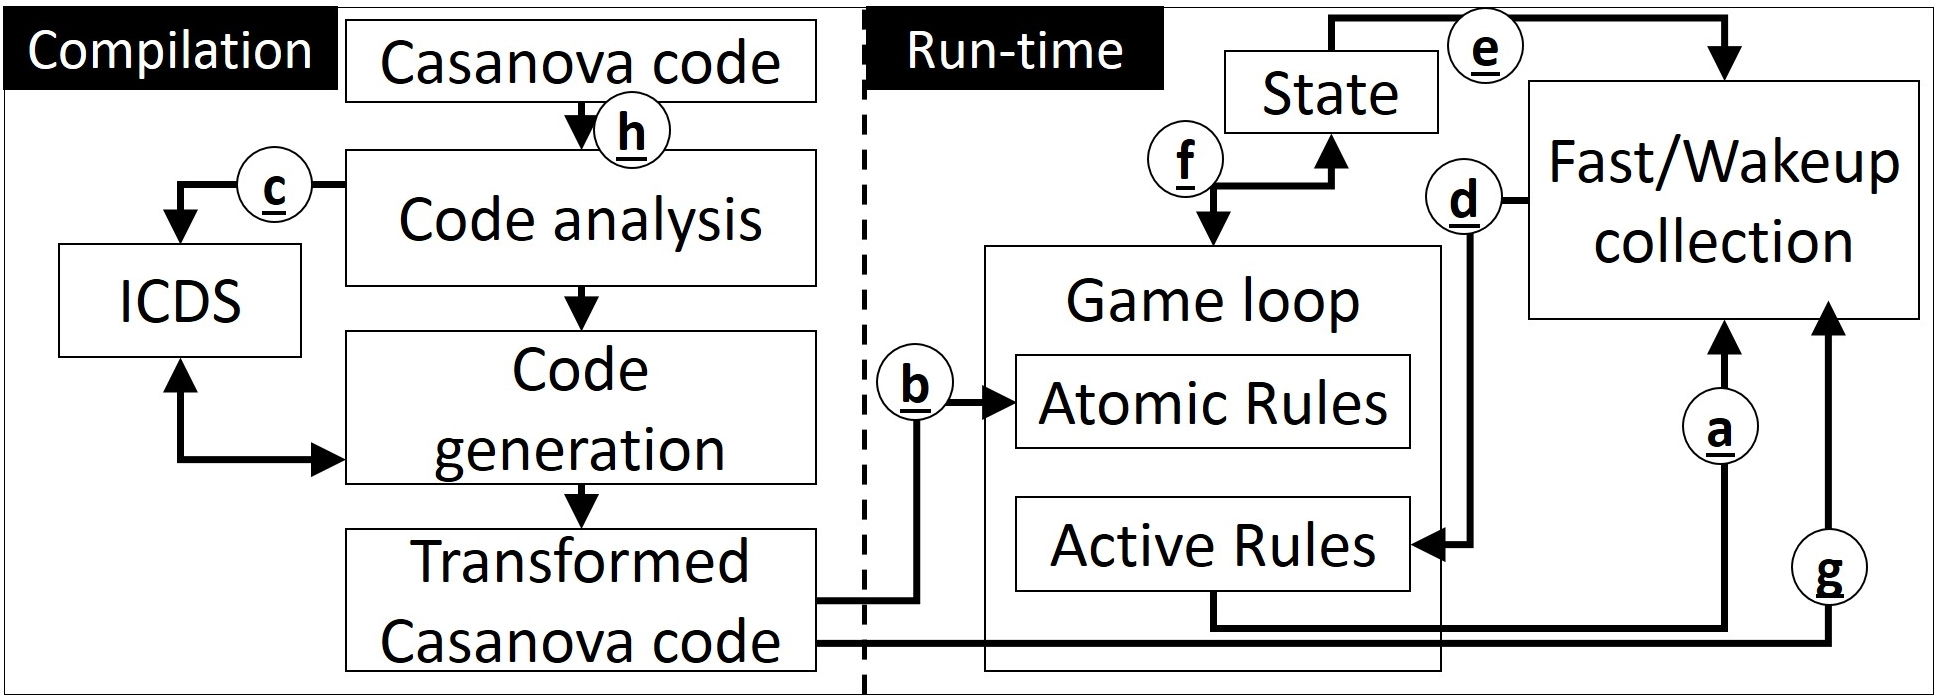
\includegraphics[scale=0.18]{Figures/system_description.jpg}
         \caption{System Configuration}
         \label{fig:system_configuration}
\end{figure}
\vspace{-10pt}


\paragraph*{Casanova overview}
Casanova is a \textit{Domain Specific Language} oriented towards game development. A program in Casanova is a set of entities organized in a tree hierarchy, of which the root is marked as \textit{world}. Each entity contains a set of fields, a set of rules, and a constructor. An extensive description of the formal grammar and semantics of Casanova can be found in \cite{maggiore2013casanova}. Casanova 2 (which we use) is a recent iteration of the original Casanova, which does not introduce changes to syntax or semantics.

In Casanova the state of a game changes only upon the execution of a \textit{rule}. A rule is a block of code acting on a subset of the entity fields called \textit{domain}, which has at least one \texttt{yield} statement and zero or more \texttt{wait} statements. The former updates the value of the fields of an entity, the latter suspends the evaluation of the rule until its condition is met, temporally affecting the fields update. The rule body is re-executed once the end is reached.

An example of a rule that illustrates the \texttt{wait} statement (which specifies that a shield is repaired when it gets damaged) is the following :
\begin{lstlisting}
rule Shields = wait Shields < 0; ...; yield Shields + 1
\end{lstlisting}
\paragraph*{Compilation - Recognizing ICs in Casanova}
From here on we will refer to the \texttt{wait} predicate as an IC, since its value affects the update of an entity with respect to the flow of time.

We also include query conditions in our IC taxonomy. We can think of a query as an entity containing a list of valid query elements that satisfy the \texttt{where} condition. An element adds itself to the valid query elements only if it satisfies the query \texttt{where} condition (this is done by adding to its rules a rule that starts with a \texttt{wait} on the query condition and ends with a \texttt{yield} that appends itself to the valid query elements).

An example of a rule with a query (which selects ships that are not destroyed) is the following:
\begin{lstlisting}
rule Ships = yield from s in Ships do
                   where s.Life > 0
                   select s
\end{lstlisting}
The effect of a \texttt{yield} is to suspend the execution of the rule for one frame and to assign the selected query elements to the selected field. To achieve the optimization as described in the previous section, the compiler uses an optimization analyzer (composed by a code analyzer and a code generator as shown in Figure \ref{fig:system_configuration}(h)), which requires the identification of ICs in code. This is discussed next.

Casanova allows interaction with external libraries and frameworks such as the .NET framework. Because the analyzer cannot infer the temporal behavior of external libraries, we add the restriction that an IC must be fully dependent on Casanova data types. The restriction is necessary because the analysis will lead to alterations in the structure of the game code and field creation, update, and access.

Given the informal considerations above, we introduce the following definitions:
\begin{inparaenum}[i)]
\item A \textit{suspendable statement} is either a \texttt{wait} or a \texttt{yield};
\item a \textit{suspendable rule} is a rule containing a suspendable statement. A suspendable rule is \textit{interesting} (ISR) if the \texttt{wait} argument is an IC or a \texttt{yield} on a query.
\item An \textit{atomic rule} is a rule which does not contain suspendable statements.
\end{inparaenum}

We now present two algorithms that respectively check if a predicate is affected by an atomic rule (Algorithm \ref{alg:atomic}) and to build the ICDS (Algorithm \ref{alg:icds_construction}). For brevity we do not present the procedure to check if a rule is an ISR, which can be done by simply looking at the syntax tree of the rule body.

\vspace{-5pt}
\begin{algorithm}
\caption{Check if a predicate is affected by an atomic rule}
\tiny
\label{alg:atomic}
\begin{algorithmic}
\Function{Atomic}{$p$}
    \State $E$ is the set of entities.
    \State $DFA \gets \emptyset$

    \For {$e \in E$}
        \State $R$ is the set of rules in $e$
        \For {$r \in R$}
            \If {$r$ is an atomic rule}
                \For{$f \in r.domain$}
                    \State $DFA \cup \lbrace (e,f) \rbrace$
                \EndFor
            \EndIf
        \EndFor
    \EndFor
    \State $D \gets$ set of $(entity,field)$ in the predicate $p$.
    \State \Return $\exists x \in D \; : \; x \in DFA$.
\EndFunction
\end{algorithmic}
\end{algorithm}
\vspace{-22pt}
\begin{algorithm}
\caption{ICDS construction}
\tiny
\label{alg:icds_construction}
\begin{algorithmic}
\Function{buildICDS}{ }
    \State $ICDS \gets \emptyset$
    \State $E$ is the set of entities.

    \For {$e \in E$}
        \State $R$ is the set of rules in $e$
        \For {$r \in R$}
            \If {$r$ is an ISR}
                \State $p$ is the first interesting condition of $r$
                \If {\textbf{not} \Call{Atomic}{$p$}}
                    \State $ICDS \cup \lbrace (e,r.index,r.domain,p) \rbrace$
                \EndIf
            \EndIf
        \EndFor
    \EndFor
    \State \Return $ICDS$
\EndFunction
\end{algorithmic}
\end{algorithm}
\vspace{-5pt}

Given a Casanova program, we build the ICDS data structure as follows: we iterate over every entity; for every rule in each entity, if the rule is suspendable, interesting and the predicate does not contain fields that are affected by an atomic rule, we add the entity, the rule index, the rule domain, and the predicate to the ICDS (See Figure \ref{fig:system_configuration}(c)).

We now focus on the identification of interesting conditions that exhibit temporal locality.

\paragraph*{Run-time efficient sleep/wake-up system}

We use the data structure generated by the analyzer to produce two distinct kinds of rules: atomic rules (see Figure \ref{fig:system_configuration}(b)) that are run every frame, and suspendable rules (see Figure \ref{fig:system_configuration}(g)). Every suspendable rule depends on an IC. %In the next section we discuss how to deal with those rules to gain higher performance.
%An idea to automatically identify entities that exhibit temporal locality is done by means of exponential regression on game entities data behavior (such as the data presented above).
Because of the property of temporal locality of rules that contain ICs, they do not need to run at every frame. Therefore the game program should activate and deactivate rules as needed at run time. The game needs to: (\textit{i}) activate a suspendable rule when its IC changes value, and (\textit{ii}) deactivate a suspendable rule when its IC is not satisfied (i.e., when it is \texttt{false}). The game keeps a rule active as long as the evaluation of its IC is \texttt{true}. Suspendable rules differ from classic atomic rules in Casanova since suspendable rules may become inactive, i.e., they do not run during every update in the game loop.

We define the \emph{Object Set} (\texttt{OBS}) as the set of pairs made of an instance of an entity and its field, that appear as arguments in an IC. Information used to build an \texttt{OBS} is collected by using the ICDS. The idea behind the optimization is that, whenever the field of an element of \texttt{OBS} changes during the game loop (see Figure \ref{fig:system_configuration}(f)), we activate the corresponding \emph{Interesting Suspendable Rule} (ISR) \texttt{R} by triggering it (see Figure \ref{fig:system_configuration}(e)).

\vspace{-0.056in}
We implement the previous behavior by means of dictionaries that keep track of the dependencies among \texttt{OBS} and \texttt{R}. We use dictionaries in this implementation since they exhibit the best asymptotic complexity with respect to the following operations: check, add, remove, and iterate. From now on we will refer these dictionaries as \emph{Dictionary of Entity-Predicate} \texttt{DEP}.

We use the static information from the ICDS (see Figure \ref{fig:system_configuration}(c)) to refer to the appropriate dictionary, based on the shape of the IC, to generate unique names for dictionaries. For every field in the predicate, we combine the name of the type of the object containing the field, the name of the field itself, the entity containing the ISR, and the ISR index.

As key we use a pair made of the reference to the object containing the field of the IC and the field itself. As value we store a collection of pairs made of the instance of the entity containing the ISR and the ISR index. We use a collection because it might be the case that one or more instances of the same entity type are pending on the same specific object field. In the example below the rule in \texttt{E} waits on a field \texttt{X} in the \texttt{world}, and the \texttt{world} contains a collection of instances of \texttt{E}. When \texttt{X} changes, all the rules of each instance of \texttt{E} waiting for \texttt{X} must be resumed.

\begin{lstlisting}
world W = X : int; L : List<E>
          rule X = wait 10; yield X + 1
          ...
entity E = ...
           rule Y = wait world.X % 2 = 0; ...
\end{lstlisting}

An entry of the dictionary in the example would be \texttt{(world,X), (L[0],rule Y)}.

\paragraph*{Suspendable rules instantiate, destroy, and update}

In order to maintain the suspendable rules we identify three stages that represent the life cycle of a suspendable rule:
\begin{inparaenum}[i)]
\item \textbf{On creation}: when we instantiate an element of which a field appears in one of the pairs of \texttt{OBS}, we use the instance and the field itself as a key to populate all its DEPs with an empty collection as value. When we instantiate an entity of which rules are targeted by an IC, we add the pair made of the entity instance and each targeted rule as a value in its DEPs;
\item \textbf{On destroy}: when an instance which appears either as a value or a key in one of DEPs, we remove all the occurrences of the instance in DEPs;
\item \textbf{On update}: when a field of an IC changes we notify the entities pending on it. After generating the IC data structure, we can safely refer to the dictionaries relying on the fact that the generated code is sound and will not produce errors at run-time. As a consequence of a notification, the ISRs involved in the notification will be activated during the next frame (if they were inactive). We add them to a collection representing the active rules of the entity containing the involved ISRs (see Figure \ref{fig:system_configuration}(d)). We group instances of the same target type into the same collection to achieve better performance (we iterate the active rules all at the same time per type instead of iterating them while iterating each entity). We store a collection in the world that contains per entity all the suspended rules that are run during a game iteration.
\end{inparaenum}


Rules in Casanova are translated at compile time into a series of switches without nesting within functions which return \texttt{void}. ISRs return \texttt{Done} when the evaluation of their IC is \texttt{false} (stay inactive) or \texttt{Working} when the evaluation of their IC is \texttt{true} (go active) or we are still busy with the execution of the block after the IC. When a suspendable rule gets suspended, i.e., its evaluation returns \texttt{Done}, we simply remove it from the active rules collection (see Figure \ref{fig:system_configuration}(a)).

\paragraph*{Query interpretation}


We transform a query into semantically equivalent code where every entity appearing in the \texttt{from} expression (\textit{source}) adds or removes itself from an index stored in the entity containing the query (\textit{target}). We add or remove a source entity in the target index only if the condition is \texttt{true}. This is done by generating a rule that waits for the condition to be \texttt{true} in the target entity. Applying our optimization to queries means that we do not need to iterate conditions every frame: we keep the rule suspended until the condition changes its value.

\begin{comment}
\paragraph*{Examples}

In the following we present three code snippets, and discuss briefly how they are interpreted by the aforementioned approach.

The first snippet below, a suspended rule update, presents the entity \texttt{E}, which contains a rule that waits until the condition \texttt{C} become \texttt{true} and a rule that updates \texttt{C} every five seconds. \texttt{C} is an interesting condition and changes only occasionally, thus the associated rule, which updates F, can benefit from optimization.
\begin{lstlisting}[frame=tlrb]{Name}
entity E =
    F  : T
    C  : bool
    rule F =
        wait C
        B
    rule C =
        wait 5.0f
        yield not C
\end{lstlisting}

The second snippet, an atomic rule update, behaves similarly to the previous one, except that \texttt{C} changes every frame. In this case \texttt{C} is an interesting condition, but the rule that changes \texttt{F} will not benefit from the optimization as \texttt{C} changes constantly.
\begin{lstlisting}[frame=tlrb]{Name}
entity E =
    F  : T
    C  : bool
    rule F =
        wait C
        B
    rule C = yield not C
\end{lstlisting}

In the third snippet, a suspended query rule update, \texttt{F} is updated by selecting those elements in \texttt{Elems} (a collection of elements of type \texttt{S}) that satisfy a condition \texttt{C}. \texttt{C} is a field in \texttt{S} which changes every five seconds.
\begin{lstlisting}[frame=tlrb]{Name}
entity E =
    F     : [T]
    Elems : [S]
    rule F =
        [for e in Elems do
         where e.C
         select e]

entity S =
    C : bool
    rule C =
        wait 5.0f
        yield not C
\end{lstlisting}

[PS: THE NEXT SENTENCE STILL DOES NOT MAKE SENSE]
Our semantics interpret the third snippet above so that to update the field \texttt{Elems}\texttt{E} only when a condition \texttt{C} is updated. We delegate the evaluation of the condition \texttt{C} to \texttt{S} so to benefit from the optimization as follows:
\begin{lstlisting}
entity E =
    F     : [T]
    Elems : [S]

entity S =
    ref SourceE : E
    C     : bool
    rule SourceE.F =
        wait C
        yield this @ SourceE.F
\end{lstlisting}
\end{comment}
% In the next section we discuss the evaluation in terms of performance and code length of our system. 

\section{Networking in Casanova 2}
\label{sec:networking}
In this section we introduce the basic concepts of the implementation of multiplayer game development for Casanova 2. This implementation aims to relieve the programmer of the complexity of hard-coding the network implementation for an online game. We show that code analysis is required to generate the appropriate network primitives to send and receive data. Finally, we present a simple multiplayer game to show a concrete example.

\subsection{Introduction}
Adding multi-player support to games is a highly desirable feature. By letting players interact with each other, new forms of gameplay, cooperation, and competition emerge without requiring any additional design of game mechanics \cite{granberg2014david}. This allows a game to remain fresh and playable, even after the single player content has been exhausted. For example, consider any modern AAA game such as \textit{Halo 4}. After months since its initial release, most players have exhausted the single player, narrative-driven campaign. Nevertheless the game remains heavily in use thanks to multiplayer modes, which in effect extended the life of the game significantly. This phenomenon is even more evident in games such as \textit{World of Warcraft} or \textit{EVE}, where multiplayer is the only modality of play and there is no single-player experience.

\paragraph{Challenges}
Multi-player support in games is a very expensive piece of software to build. Multiplayer games are under strong pressure to have very good \textit{performance}\cite{claypool2006latency}. Performance is both in terms of CPU time, and in bandwidth used. Also, games need to be very \textit{robust} with respect to transmission delays, packets lost, or even clients disconnected. To make matters worse, players often behave erratically. It is widespread practice among players to leave a competitive game as soon as their defeat is apparent (a phenomenon so common to even have its own name: ``rage quitting'' \cite{rage_quitting}), or to try to abuse the game and its technical flaws to gain advantages or to disrupt the experience of others.

Networking code reuse is quite low across titles and projects. This comes from the fact that the requirements of every game vary significantly: from turn-based games that only need to synchronize the game world every few seconds, and where latency is not a big issue, to first-person-shooter games where prediction mechanisms are needed to ensure the smooth movement of synchronized entities, to real-time-strategy games where thousands of units on the screen all need to be synchronized across game instances \cite{smed2002aspects}. In short, previous effort is substantially inaccessible for new titles. Encapsulation suffers from this ad-hoc nature of the implementation of the networking layer in multiplayer games. Indeed managing the information about game updates over a network requires each game entity to interface the game logic code with network connection and socket objects, data transmission method calls such as send and receive, and support data structures to manage traffic and track the status of common protocols. This happens because each game entity must provide the following functionality in order to work in a multiplayer game:

\begin{itemize}
	\item Update the logic in the fashion of a singleplayer counterpart.
	\item Choose what data is necessary to send over the network and create the message containing this information.
	\item Choose what data can be lost and what data must always be received by the other clients.
	\item Periodically check if incoming messages contain information which needs to be read and to specific updates.
\end{itemize}

Combining these requirements together within the same entity breaks encapsulation because now the logic of the entity and lots of spurious details only relevant to the networking implementation are mixed together, resulting in a highly noisy program. Maintenance then becomes very hard, as every change in the game logic must also be reflected in the networking implementation.

\paragraph{Existing approaches}
Networking in games is usually built with either very low-level or very high-level mechanisms. Very low-level mechanisms are based on manually sending streams of bytes and serializing only the essential bits of the game world, usually incrementally, on unreliable channels (UDP). This coding process is highly expensive because building by hand such a low-level protocol is difficult to get right, and debugging subtle protocol mismatches, transmission errors, etc. will take lots of development resources. Low-level mechanisms must also be very robust, making the task even harder.

High-level protocols such as RDP, reflection-based serialization, etc. can also be used. These methods greatly simplify networking code, but are rarely used in complex games and scenarios. The requirements of performance mean that many high-level protocols or mechanisms are insufficient, either because they are too slow computationally (especially when the rely on reflection) or because they transmit too much data across the network.

\subsection{Motivation}

To avoid the problems of both existing approaches, we propose a middle ground. We observe that networking fundamental abstractions upon which the actual code and protocols are built do not vary substantially between games, even though the code that needs to be written to implement them does. The similarity comes from the fact that the ways to serialize, synchronize, and predict the behaviour of entities are relatively standard and described according to a limited series of general ideas. The difference, on the other hand, comes from the fact that low-level protocols need to be adapted to the specific structure of the game world and the data structures that make it up. Until now, common primitives have not been syntactically and semantically captured inside existing domain-specific languages for game development\cite{bhatti2009domain}. Using the right level of abstraction, these general patterns of networking can be captured, while leaving full customization power in the hand of the developer (to apply such primitives to any kind of game).




\section{Networking architecture}
\label{sec:net_architecture}
In this section we introduce a small example that addresses the requirements of designing a multiplayer game. We then present an architecture that aims to fulfil these requirements.

\subsection{The master/slave network architecture}

We chose to implement the networking layer in Casanova 2 by using a peer-to-peer architecture for the following reasons:

\begin{itemize}
	\item Server-client architectures are more reliable but suitable only for specific genres of games (mostly Shooter games), while other genres, such as Real-time strategy games or Online Role Playing Games use P2P architectures.
	\item We do not have to write a separate logic for an authoritative game server, which has to validate the actions of clients.
\end{itemize}

Casanova will provide a generic tracking server, which is run separately from the main program. The tracking server is a thin service that connects players participating in a single game, and helps with forwarding the network traffic through NATs.

Each client maintains a local copy of the \texttt{world} entity and has direct control over a single portion of it. Instances belonging to such as portion are seen as \textit{master} by this player, who is always allowed to directly change the state of the master instances without having to validate this state change by synchronizing with other players through the network.

Each client also maintains a portion of the world that is not directly under his control. Instances belonging to such as portion are seen as \textit{slave} by this player, who is only allowed to \textit{predict} the local state of the instances and, whenever he receives an update from their masters, must correct this prediction according to the data contained in the received messages. The slave part of the world is thus maintained passively by the client: the only active part is predicting the evolution of the entity state and correcting it whenever he receives an update by its master.

For this purpose we extend the syntax of Casanova rules by allowing them to be marked with the modifiers \texttt{master} and \texttt{slave}. These rules are executed respectively on master and slave entities. Note that it is still possible not to mark a rule with these modifiers, which means that the rule is always executed independently of the fact that the entity is either master or slave on that particular client. We also allow to mark a rule as \texttt{connecting} and \texttt{connected}. These rules are triggered only once respectively when a new client connects and when the clients detect a new connection.

Casanova also provides primitives to send (reliably or unreliably) and receive data. A schematic representation of this architecture can be seen in Figure \ref{fig:masterslave}.

\begin{figure}[h!]
	\centering
	\caption{Representation of the game world in a networking scenario}
	\label{fig:network_world}
	\begin{subfigure}[t]{0.3\linewidth}
		\centering
		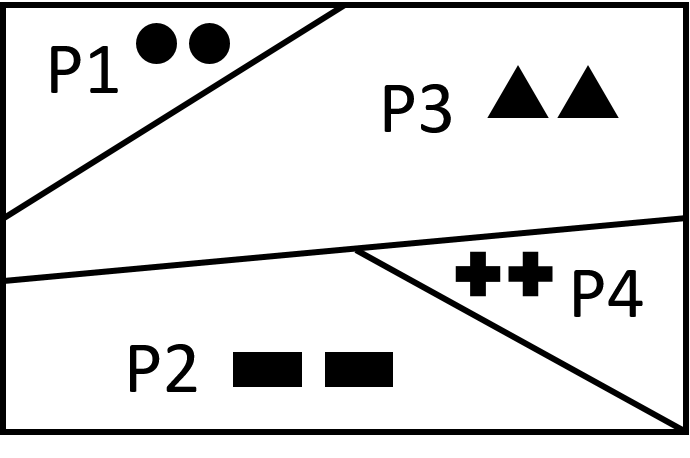
\includegraphics[width=1\linewidth]{Figures/networking2}
		\caption{Unknown correct game state when P3 joins the game.\\}
		\label{subfig:networking_ideal}
	\end{subfigure}
	\begin{subfigure}[t]{0.3\linewidth}
		\centering
		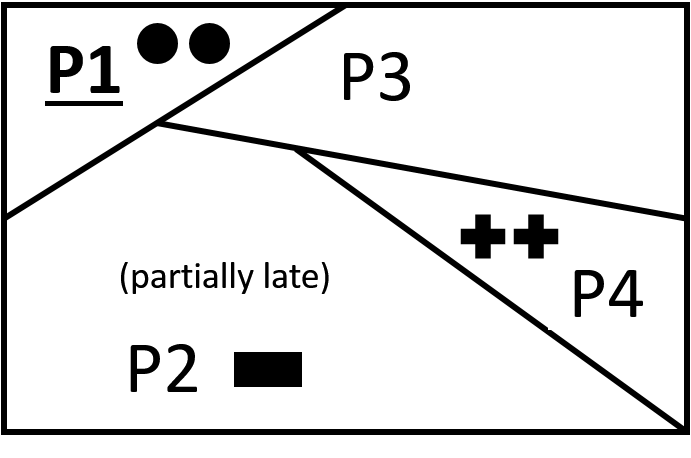
\includegraphics[width=1\linewidth]{Figures/networking1}
		\caption{Networking game state seen from the point of view of P1. P2 is partially synchronized, P4 is fully synchronized, and P3 is a new client that is late and is still sending its data}
		\label{subfig:networking_relative}
	\end{subfigure}
	

\end{figure}

\begin{figure}
	\centering
	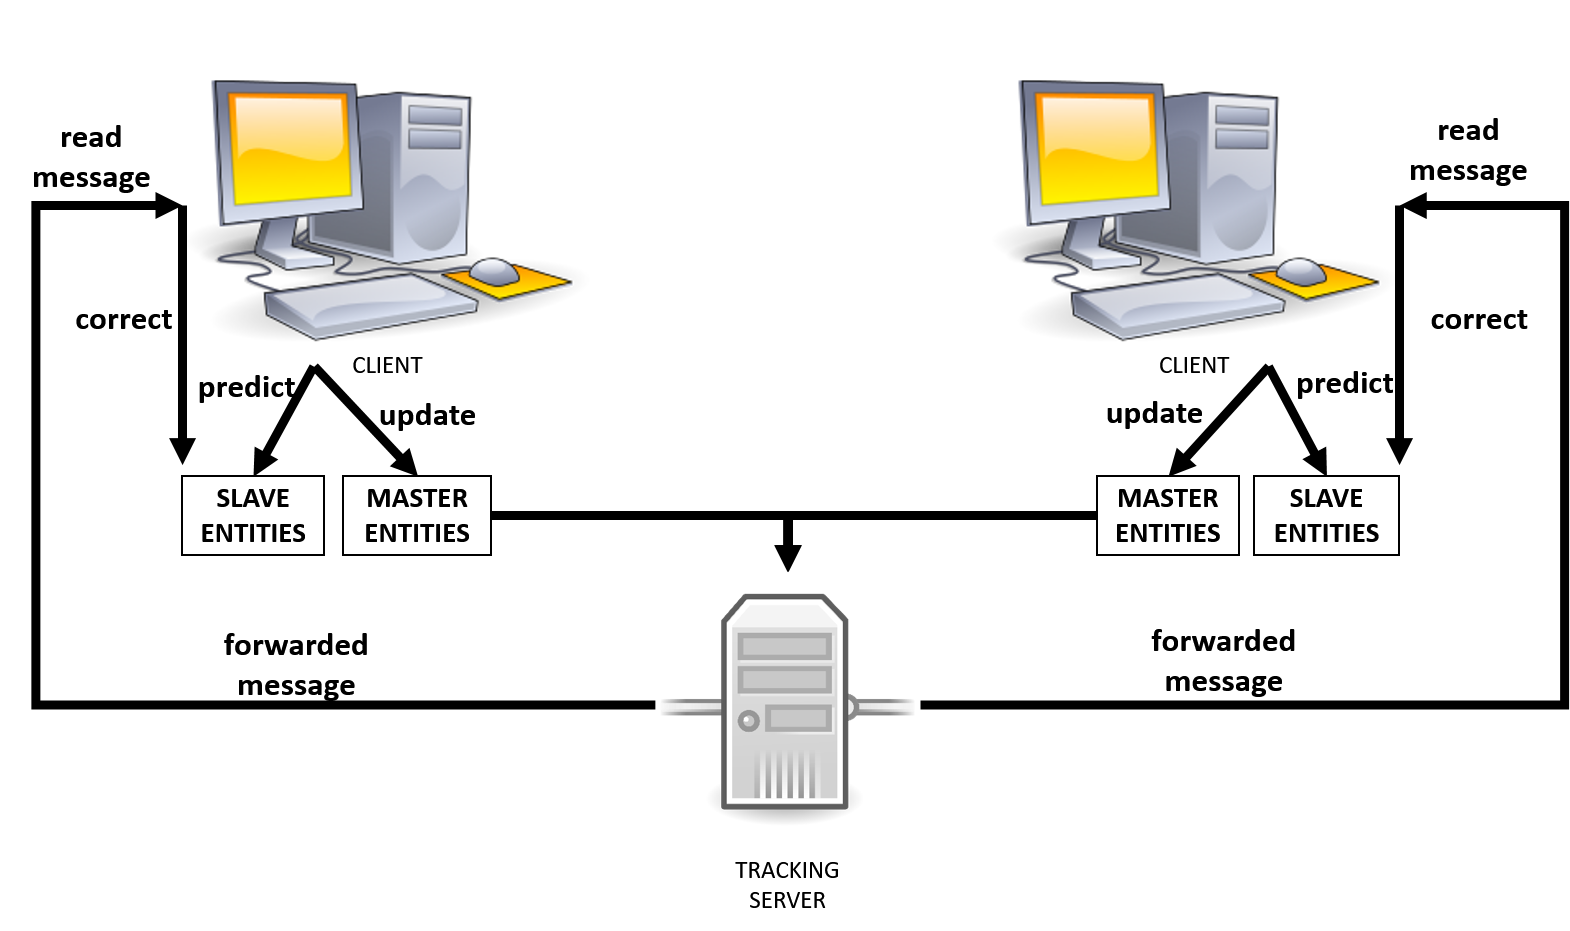
\includegraphics[scale = 0.5]{Figures/masterslave}
	\caption{master/slave architecture}
	\label{fig:masterslave}
\end{figure}

Note the aim of this architecture is to provide language-level primitives to describe the networking logic. This means that the compiler will be able to generate code compatible with the low-level network libraries that provide transmission functions over the network channel without having to change Casanova code in the program. In our implementation we chose the .NET library \texttt{Lidgren}, which is widely used also in commercial game engines, such as Unity3D and MonoGame, but nothing prevents the compiler to be expanded in order to target other similar libraries for other languages, such as jgroups \cite{ban2002jgroups}.

\subsection{Case study}
Let us consider a simple shooter game where each player controls a space ship. Players can move forward, backward, and rotate the ship to change direction. Moreover, they can use the ship lasers to shoot other players. If a laser hits an enemy ship we increase the player's score. Designing such a game requires to address the following issues, depicted by the schematic representation in Figure \ref{fig:network_world}:

\begin{enumerate}
	\item Each player must maintain a local version of the game state (world). In order to avoid to flood the network with messages, all the copies are not fully synchronized at each frame, thus they are slightly different and each client knows the latest version of only part of the copy.
	\item A player \texttt{connecting} to an existing game must be able to receive the latest update of the game state and send the new ship he will control to existing players in the game.
	\item A player already \texttt{connected} to the game must detect a new connection and send his master portion of the game state.
	\item Each player must be able to control only one ship at a time. This means that the part of the game logic that processes the input and modifies the spatial data of the ship (position and rotation) should only be executed on the ship controlled by the player and not on the local copies of other players' ships. This means that each player sees as \texttt{master} only one ship instance.
	\item Each player must send the updated state of the ship he controls to the other players after executing the local update. To achieve better performance over the network, the data is not sent at every update, but with a lower frequency.
	\item Each player must receive the updated state of \texttt{slave} ships controlled by other players. In this phase we must take into account that, as explained above, not every update is sent so the player should ``predict'' what will happen during the game frames in which he does not receive an update.
\end{enumerate}

\subsection{Implementation}
Each of the scenarios described above requires specific language extensions. These extensions identify connection, ownership (master/slave), and various send and receive primitives. In this section we introduce each primitive by using a multiplayer game example \footnote{The game source code and executable can be found at \url{https://github.com/vs-team/casanova-mk2/wiki/Networking-extension}}. We now give an implementation of the shooter game presented above and using the extended version of Casanova 2 with network primitives. 

The \texttt{world} contains a list of ships controlled by each player.
\begin{lstlisting}
world Shooter = {
  Ships  : [Ship]
  ...
}
\end{lstlisting}

Each \texttt{Ship} contains a position, a rotation, a collection of shot projectiles, and the score.
\begin{lstlisting}
entity Ship = {
  Position   : Vector2
  Rotation   : float32
  Projectiles : [Projectile]
  Score		  : int
  ...
}

\end{lstlisting}

Each \texttt{Projectile} contains its position and velocity.

\begin{lstlisting}
entity Projectile = {
  Position : Vector2
  Velocity : Vector2
  ...
}
\end{lstlisting}

\subsubsection{Connection}
When a player connects we must consider two different situations: (\textit{i}) a player is already in the game and must send the current game state to the connecting players, and (\textit{ii}) the player who is connecting needs to send the ship he will instantiate and control (its initial state). Both the players in the game and the connecting one must receive the game states that are sent. For this purpose we introduce two additional modifiers, \texttt{connecting} and \texttt{connected}, that can be added to rule declarations to mark their role in the multiplayer logic.

\paragraph{Connecting:} A rule marked with \texttt{connecting} is executed once when a player joins the game for the first time. In our example the player should send his initial state (the created ship) to the other players. We use the primitive \texttt{send\_reliable} because we must be sure that eventually all players will be notified of the ship creation.
	\begin{lstlisting}
world Shooter = {
  ...
  rule connecting Ships =
    yield send_reliable Ships
}
	\end{lstlisting}
	
\paragraph{Connected:} A rule marked with \texttt{connected} is run whenever a new player joins the game by all existing players. When this occurs, each player sends its ship. The system will take care to send only the ship controlled locally by the player itself for each player. The rule will use the \texttt{send\_reliable} primitive for the same reason explained in the previous point.

\begin{lstlisting}
world Shooter = {
  ...
  rule connected Ships =
    yield send_reliable Ships
}
\end{lstlisting}

Note that even if the code is the same, the semantics of the two rules are different. The first one is executed by the player joining the game, who locally instantiates its \texttt{Ship} and must send its list of \texttt{Ships} (containing only the local instance) to the other players. The second one is executed by all existing players who must share with the joining player the list of existing ships.


\subsubsection{Master updates}
As explained above, each client manages a series of local game objects (called \textit{master objects}) that are under its direct control. The other clients read passively any update done on those instances and update their remote copy  (\textit{slave objects}) accordingly. We mark rules affecting the behaviour of master objects as \texttt{master}. In our example the following situations are run as master: (\textit{i}) synchronizing the ships among players, (\textit{ii}) updating the ship and projectiles spatial data, and (\textit{iii}) creating and destroying projectiles.

\begin{enumerate}
	\item Each player is tasked to maintain the list of Ships in the world. This requires to receive the updated list from other players and to store the new value in a master rule. Indeed the world is a special case of an entity that is shared among players, and not directly owned by somebody. Each ship contained in that list and received from other players will be treated appropriately as slaves, while the only one owned by the current player will be under his direct control. In this rule we use \texttt{let!}, which is an operator that waits until the argument expression returns a result and then binds it to the variable. The symbol \texttt{@} stands for list concatenation. The rule uses \texttt{receive\_many}, which receives and collects the list of sent ships by the other players.
	
	\begin{lstlisting}
world Shooter = {
  ...
  rule master Ships =
    let! ships = receive_many()
    yield Ships @ ships
}
	\end{lstlisting}
	
	\item The master version of the ship update reads the input of the player and moves (or rotates) the ship if the appropriate key is pressed. Note that this part must be executed only on a master object, because we want to allow each player to control only the ship it owns and instantiates at the beginning of the game. Below we show just the rule to move forward; the other movement and rotation rules are analogous. We use an \textit{unreliable send} because it is acceptable to lose an update of the position during a certain frame: shortly after there will be a new update.
	
	\begin{lstlisting}
entity Ship = {
  ...
  rule master Position =
    wait world.Input.IsKeyDown(Keys.W)
    let vp = new Vector2(Math.Cos(Rotation), 
                         Math.Sin(Rotation)) * 300.0f
    let p = Position + vp * dt
    yield send p
}
	\end{lstlisting}
	
	We do the same for projectiles, except the projectile position is continuously updated and synchronized over the network without having to wait that a key is pressed.
	
	\item Creating a new projectile happens when the player shoots. A ship keeps track of the projectiles it has shot so far, and adds a new one to the list of the existing projectiles. The updated list is sent to all players with the new instance of the projectile. As explained in Section \ref{sec:net_architecture}, we only send the new projectiles and not the whole list. Note that the last \texttt{wait} forces the player to release the key before shooting again (semi-automatic fire). Removing that check would spawn multiple projectiles consecutively, which is not a wanted behaviour.
	
\begin{lstlisting}
entity Ship = {
  ...
  rule master Projectiles =
    wait world.Input.IsKeyDown(Keys.Space)
    let vp = new Vector2(Math.Cos(Rotation), 
                         Math.Sin(Rotation)) * 500.0f
    let projs = new Projectile(Position, vp) :: Projectiles
    yield send_reliable projs
    wait not world.Input.IsKeyDown(Keys.Space)
}
\end{lstlisting}

	Filtering the colliding projectiles and updating the score is run as a master rule. The rule computes the set difference between the ship projectiles and the colliding projectiles and updates the list of projectiles, sending them through the network as well. Even in this case, the network layer sends only the information about the projectiles to remove. Note that the score is managed by each player locally, as it does not require to be synchronized (we do not print the other players' scores. Doing so would indeed require to also send the score).
	
\begin{lstlisting}
entity Ship = {
  ...
  rule master Projectiles, Score =
    let collidingProjs =
      [for p in Projectiles do
       let ships =
         [for s in Ships do
          where 
           s <> this and 
           Vector2.Distance(p.Position,s.Position) < 100.0f
          select s]
       where ships.Count > 0
       select p]
    let newProjectiles = Projectiles - collidingProjs
    yield send_reliable newProjectiles, 
          Score + collidingProjs.Count 
}
\end{lstlisting}
\end{enumerate}

\subsubsection{Managing remote instances}
The game objects that were not instantiated by a client, but received from another client, are \textit{slave objects} and must be synchronized differently than master objects. For this purpose, a rule can be marked as \texttt{slave}. In our example we use slave rules in the following situations: (\textit{i}) synchronizing other players' ships and projectiles spatial data, and (\textit{ii}) projectiles instantiated by other players.

\begin{enumerate}
	\item Every remote projectile and ship is synchronized locally by a rule, which tries to \texttt{receive} a message containing updated spatial data. Below we provide the code to update the position of the ship; the synchronization of other spatial data is analogous.
	
\begin{lstlisting}
  entity Ship = {
  ...
  rule slave Position = yield receive()
}
\end{lstlisting}
	
	\item When a projectile is instantiated remotely, we have to receive it and add it to the list of projectiles. We use \texttt{receive\_many} because the new projectiles are added to a list. This case also supports the situation where a ship could shoot multiple projectiles at the same time.
	
\begin{lstlisting}
entity Ship = {
  ...
  rule slave Projectiles =
    let! projs = receive_many()
    yield projs @ Projectiles
}
\end{lstlisting}
\end{enumerate}

In this scenario is important to discuss the atomicity of these transmissions: in the context of network games, reliability is often sacrificed for better network performance, so most of the data transmissions are unreliable (like in the case of the ship position). This means that we have no guarantee that the message will be received. Several issues can arise from this situation: for example, if a player fails to receive the position of the ship then it might miss a collision with a projectile. This is a well-known issue in several shooter games and out-of-sync errors might happen during a multiplayer game. However, ensuring that all the data transmissions are reliable might affect network performance to the point that the game would become unplayable because of the network overload. Casanova 2 allows the programmer to decide whether the transmission should be reliable or not and experiment with the effect of a reliable transmission versus an unreliable one that does not overload the network. For example, the updated list of projectiles, after a collision, is always sent in a reliable way. This is acceptable because collisions are not so frequent. This is not true for the ship position, since movements are very frequent and mostly happen at every frame, thus it is something that should not be sent reliably at every frame.




\section{Evaluation}
\label{sec:evaluation}
In this section we evaluate the performance of our approach. A comparison on the same Casanova game code between the non-optimized implementation, the optimized one, and an implementation in C\#, will be shown and discussed in terms of run-time performance and code complexity.

\subsection{Experimental setup} In order to get a systematic evaluation of the proposed approach to encapsulation, a generic game is considered, in which a group of entities are spawned every \texttt{K} seconds and stay inactive for a random amount of time, between 5 and 10 seconds. Then they are activated and start moving for a randomly determined amount of time, between 4 and 8 seconds. Finally, they are destroyed, by triggering a condition in the entities. For the evaluation, additional conditions are added (with different timers), in order to make the simulation dynamics more articulated and ``heavy'' in terms of amount of code to run.


In this experiment, we compare the code generated by the Casanova compiler versus our optimization built in the Casanova compiler, and an idiomatic implementation in the C\# language (a commonly-used language for building games). We also ran the games with two different front ends, namely Unity3D and MonoGame, both using .NET.
For each test we measure the time (in milliseconds) that the game takes to fully complete a game iteration (i.e., updating all the entities in the game). We did not include the time it takes to render the game screen, since rendering is not affected by our optimization, though it might affect the performance measure.
\subsection{Performance evaluation} Table \ref{tab:times} shows the performance results. As we can see, in both cases, the performance of our optimized Casanova 2 code is higher than the one of non-optimized implementation, and the idiomatic C\# implementation. Using Unity3D, the optimized code is one order of magnitude faster than the non-optimized code. Using MonoGame, the optimization is faster but on the same order of magnitude. The difference is due to the implementation of the underlying frameworks.

\begin{table}[!ht]
\caption{Code lines comparison for a singleplayer game}
\label{tab:length}
\centering
\begin{tabular}{ @{}|c|c|c|c|@{} }
\hline
  Original language & Generated language & Optimized code & Lines \\ \hline
  Casanova & - & - & 45 \\
  Casanova & C\# & No & 139 \\
  Casanova & C\# & Yes & 327 \\
  C\# & - & - & 88 \\ \hline
\hline
\end{tabular}
\end{table}

\begin{table}
\caption{Running time comparison for a singleplayer game}
\label{tab:times}
\centering
\begin{tabular}{ @{}|c|c|c|c|@{} }
\hline
 Platform & Language & Optimized & Performance\\ \hline
\multirow{3}{*}{Monogame}
  & Casanova & No & 0.0159 ms\\
  & Casanova & Yes & 0.0098 ms\\
  & C\# &   - & 0.0147 ms\\ \hline
\multirow{3}{*}{Unity3D}
  & Casanova & No & 0.0257 ms\\
  & Casanova & Yes & 0.0085 ms\\
  & C\# &   - & 0.1642 ms\\ \hline
\hline
\end{tabular}
\end{table}

\begin{table}
\caption{Code lines comparison for a multiplayer game}
\centering
\label{tab:networking}
\centering
\begin{tabular}{ @{}|c|c|@{} }
	\hline
	Language & Lines \\ \hline
	Casanova & 126 \\
	\hline
	C\# &  1257 \\
	\hline
\end{tabular}
\end{table}

\subsection{Code size evaluation}
Table \ref{tab:length} shows the code length for each implementation. Casanova 2 game code needs about half the lines of code compared to the idiomatic C\# implementation for single player games. When comparing networking code, the difference is one order of magnitude (see Table \ref{tab:networking}). The intermediate code that the Casanova 2 compiler creates (which is C\# code) is considerably longer due to the presence of support data structures. With increasing code complexity, we may expect the original Casanova 2 code to remain compact, while the generated code will increase rapidly in size, with additional data structures and associated logic code. Writing such optimized code by hand is a daunting and expensive task.

\section{Conclusions}
\label{sec:conclusions_and_future_works}
Game developers often have to choose between maintainability of their code and speed of execution, a choice that more often than not favors speed over maintainability. By using encapsulation, game code may be written in a maintainable way, but compilation of encapsulated code in general-purpose languages often leads to slower games. We proposed a solution to the loss of performance in encapsulated programs using automated optimization at compile time. 
We presented an implementation of this solution in the Casanova 2 language. We showed that our approach transforms encapsulated code, through extensive automated optimization, into a high-performance executable that easily rivals the speed of a C\# implementation. Moreover, we showed that Casanova 2 code needs about half the lines of code as the C\# implementation, with even more dramatic results if we consider well-known complex and verbose network code: good primitives for networking preserve encapsulation because they do not require polluting the identity of an entity with network specific information that it is not related to the game logic of the entity itself. Of course networking does impact the logic of the entity, but this should be reflected by minimal code adjustments. Our research, which is still in its initial stage, requires more (and more complex) samples and further investigation. Still, preliminary experiments suggest that our approach allows game developers to write clear, readable code, which is both high-performance and maintainable. 

In the near future, we will add a dynamic analysis of the game to automatically identify entities that exhibit temporal locality. Such an analysis must be done while playing the game to keep track of the amount of time that each rule stays inactive, and periodically the game must be recompiled to generate or remove the optimization code for an entity based on the temporal information generated by the analyser. 

Furthermore, we are actively developing a meta-compiler that generates predictable, high-performance code that makes very little to no use of dynamic constructs. A meta-compiler is a software that takes as input the definition of a programming language and a program written in that language and outputs executable code. This meta-compiler features a programmable, higher-kinded type system that feeds an aggressive code inliner. Our meta-compiler is designed to be agnostic with respect to the architecture of one's library for generating code: it could be used for Aspect-Oriented Programming, the inlining of monad transformers, query optimizations, and even other forms of static code analysis such as abstract interpretation or model checking. Such work is unfortunately very complex and as such is not yet in a state to be used in practice with the results of the current paper. We plan on rebuilding the existing Casanova compiler, and all of its optimizations, within the meta-compiler itself. A preliminary result can be found in \cite{meta_casanova}.


%\paragraph*{Future work}

%As seen in Algorithm \ref{alg:icds_construction} of Section \ref{sec:details}, in the current implementation only the first IC of a rule is considered for the optimization process. A further improvement to the optimizer is to use multiple ICs for the same rule. This requires a refinement of the mechanism of dictionaries to keep track at what IC the rule was halted.

%Furthermore, in the near future we will add a dynamic analysis of the game to automatically identify entities that exhibit temporal locality, to avoid developers having to indicate those entities by hand. Such an analysis must be done while playing the game to keep track of the amount of time that each rule stays inactive, and periodically the game must be recompiled to generate or remove the optimization code for an entity based on the temporal information generated by the analyzer. 


\begin{comment}





%%%%%%%%%%%%%%%%%%%%%%%%%%%%%%%%%%%%%%%%%%
\section{Results}

This section may be divided by subheadings. It should provide a concise and precise description of the experimental results, their interpretation as well as the experimental conclusions that can be drawn.

%%%%%%%%%%%%%%%%%%%%%%%%%%%%%%%%%%%%%%%%%%
\subsection{Subsection}
\subsubsection{Subsubsection}

Bulleted lists look like this:
\begin{itemize}[leftmargin=*,labelsep=4mm]
\item	First bullet
\item	Second bullet
\item	Third bullet
\end{itemize}

Numbered lists can be added as follows:
\begin{enumerate}[leftmargin=*,labelsep=3mm]
\item	First item
\item	Second item
\item	Third item
\end{enumerate}

The text continues here.

\subsection{Figures, Tables and Schemes}

All figures and tables should be cited in the main text as Figure 1, Table 1, etc.

\begin{figure}[H]
\centering
%
\includegraphics[width=3cm]{logo-mdpi}
\caption{This is a figure, Schemes follow the same formatting. If there are multiple panels, they should be listed as: (\textbf{a}) Description of what is contained in the first panel. (\textbf{b}) Description of what is contained in the second panel. Figures should be placed in the main text near to the first time they are cited. A caption on a single line should be centered.}
\end{figure}   

All figures and tables should be cited in the main text as Figure 1, Table 1, etc. All figures and tables should be cited in the main text as Figure 1, Table 1, etc. All figures and tables should be cited in the main text as Figure 1, Table 1, etc. All figures and tables should be cited in the main text as Figure 1, Table 1, etc.

\begin{table}[H]
\caption{This is a table caption. Tables should be placed in the main text near to the first time they are cited.}
\small % Font size can be changed to match table content. Recommend 10 pt by default.
\centering
\begin{tabular}{ccc}
\toprule
\textbf{Title 1}	& \textbf{Title 2}	& \textbf{Title 3}\\
\midrule
entry 1		& data			& data\\
entry 2		& data			& data\\
\bottomrule
\end{tabular}
\end{table}

\subsection{Formatting of Mathematical Components}

This is an example of an equation:

\begin{equation}
\mathbb{S}
\end{equation}

%% If the documentclass option "submit" is chosen, please insert a blank line before and after any math environment (equation and eqnarray environments). This ensures correct linenumbering. The blank line should be removed when the documentclass option is changed to "accept" because the text following an equation should not be a new paragraph. 
Please punctuate equations as regular text. Theorem-type environments (including propositions, lemmas, corollaries etc.) can be formatted as follows:
%% Example of a theorem:
\begin{Theorem}
Example text of a theorem.
\end{Theorem}
The text continues here. Proofs must be formatted as follows:

%% Example of a proof:
\begin{proof}[Proof of Theorem 1]
Text of the proof. Note that the phrase `of Theorem 1' is optional if it is clear which theorem is being referred to.
\end{proof}
The text continues here.

%%%%%%%%%%%%%%%%%%%%%%%%%%%%%%%%%%%%%%%%%%

\section{Discussion}

This section may be divided by subheadings. Authors should discuss the results and how they can be interpreted in perspective of previous studies and of the working hypotheses. The findings and their implications should be discussed in the broadest context possible. Future research directions may also be highlighted.

%%%%%%%%%%%%%%%%%%%%%%%%%%%%%%%%%%%%%%%%%%

\section{Materials and Methods}

This section should be divided by subheadings. Materials and Methods should be described with sufficient details to allow others to replicate and build on published results. Please note that publication of your manuscript implicates that you must make all materials, data, and protocols associated with the publication available to readers. Please disclose at the submission stage any restrictions on the availability of materials or information. New methods and protocols should be described in detail while well-established methods can be briefly described and appropriately cited.

Research manuscripts reporting large datasets that are deposited in a publicly available database should specify where the data have been deposited and provide the relevant accession numbers. If the accession numbers have not yet been obtained at the time of submission, please state that they will be provided during review. They must be provided prior to publication.

%%%%%%%%%%%%%%%%%%%%%%%%%%%%%%%%%%%%%%%%%%

\section{Conclusions}

This section is not mandatory, but can be added to the manuscript if the discussion is unusually long or complex.

%%%%%%%%%%%%%%%%%%%%%%%%%%%%%%%%%%%%%%%%%%
\vspace{6pt}  %%MDPI internal note: new layout%%
%% optional
\supplementary{\textbf{Supplementary Materials:} The following are available online at www.mdpi.com/link, Figure S1: title, Table S1: title, Video S1: title.}  %%MDPI internal note: new layout%%

%%%%%%%%%%%%%%%%%%%%%%%%%%%%%%%%%%%%%%%%%%

\acknowledgments{\textbf{Acknowledgments:} All sources of funding of the study should be disclosed. Please clearly indicate grants that you have received in support of your research work. Clearly state if you received funds for covering the costs to publish in open access.}

%%%%%%%%%%%%%%%%%%%%%%%%%%%%%%%%%%%%%%%%%%

\authorcontributions{\textbf{Author Contributions:} For research articles with several authors, a short paragraph specifying their individual contributions must be provided. The following statements should be used ``X.X. and Y.Y. conceived and designed the experiments; X.X. performed the experiments; X.X. and Y.Y. analyzed the data; W.W. contributed reagents/materials/analysis tools; Y.Y. wrote the paper.'' Authorship must be limited to those who have contributed substantially to the work reported.}

%%%%%%%%%%%%%%%%%%%%%%%%%%%%%%%%%%%%%%%%%%
\end{comment}

\conflictofinterests{\textbf{Conflicts of Interest:} Declare conflicts of interest or state ``The authors declare no conflict of interest.'' Authors must identify and declare any personal circumstances or interest that may be perceived as inappropriately influencing the representation or interpretation of reported research results. Any role of the funding sponsors in the design of the study; in the collection, analyses or interpretation of data; in the writing of the manuscript, or in the decision to publish the results must be declared in this section. If there is no role, please state ``The founding sponsors had no role in the design of the study; in the collection, analyses, or interpretation of data; in the writing of the manuscript, and in the decision to publish the results''.} 


%=================================================================
% References: Variant A
%=================================================================
% Back Matter (References and Notes)
%----------------------------------------------------------
% Style and layout of the references
\bibliographystyle{mdpi}
\renewcommand\bibname{References}
%%MDPI internal note: new layout%% redefinition removed

\begin{comment}


\begin{thebibliography}{999} %%MDPI internal note: new layout%% always leave 999
% Reference 1
\bibitem{ref-journal}
Lastname, F.; Author, T. The title of the cited article. {\em Journal Abbreviation} {\bf 2008}, {\em 10}, 142-149.

% Reference 2
\bibitem{ref-book}
Lastname, F.F.; Author, T. The title of the cited contribution. In {\em The Book Title}; Editor, F., Meditor, A., Eds.; Publishing House: City, Country, 2007; pp. 32-58.

\end{thebibliography}
\end{comment}
%=================================================================
% References:  Variant B
%=================================================================
% Use the following option to include external BibTeX files:

\bibliography{references}
\bibliographystyle{mdpi}



\end{document}

